
\documentclass[a4paper,11pt]{report} %%%% sytle du document : report/book/article


\usepackage[utf8]{inputenc} %% pour les accents en français
\usepackage[frenchb]{babel} %% pour un format français
\usepackage{graphicx} %% pour afficher des graphiques
\usepackage{amsmath} %% pour écrire des symboles (maths), des équations, etc.
\usepackage{amssymb}
\usepackage{color}
\usepackage{bm} %% pour lister des citations/la biblio
\usepackage{hyperref} %% pour inserer des liens internet
\usepackage{cleveref} %% pour faire des références uax équations, tableaux, etc.
%\usepackage{setspace} %% pour changer l'espace entre les lignes
%\linespread{1.6} %% pour changer l'espace entre les lignes



\setcounter{chapter}{1}

%%%%%%%%%%%%%%%%%%%%%%%%%%%%%%%%%%%%%%%%%%%%%%%%%%%%%%%%%%%%%%%%%%%%%%%%%%%%%%%
\title{\textbf{Ecoulement potentiel 2D}} %% choissez un titre approprié à votre sujet
\author{par\\CISCARD Julie\\ZHANG Xunjie\\pour le TP3 de l'UE éléments finis M1} %% utilisez \\ pour une nouvelle ligne
\date{fait le 29 novembre 2016} %% pour afficher la date actuelle commenter cette ligne


%%%%%%%%%%%%%%%%%%%%%%%%%%%%%%%%%%%%%%%%%%%%%%%%%%%
%%TOUT ce qui va dans votre rapport doit être entre \begin{document} & \end{document}
\begin{document}
\selectlanguage{french} %% format français
\maketitle %% pour afficher le titre
\tableofcontents %% pour afficher/compiler le sommaire automatiquement
\listoffigures %% pour lister les figures
\pagebreak

%%%%%%%%%%%%%%%%%%%%%%%%%%%%%%%%%%%%%%
\section{Introduction}

\subsection{Objectif}

L'objectif de ce TP est d'utiliser la méthode des éléments finis pour un problème physique en 2 dimensions. Le problème physique étudié ici est l'écoulement potentiel dans un canal avec un obstacle.\\

Ce Travail Pratique peut avoir comme application les exemples suivant:
\begin{itemize} 
   \item un cours d'eau avec un rocher comme obstacle;
   \item un canal aboutissant sur une écluse où l'eau arrive est le bateau est considéré comme un obstacle;
\end{itemize}

Nous devons donc à l'aide des condition aux limites, à la fonction de courant $\psi$, et à l'équation de Bernouilli déterminer la pression ainsi que la vitesse dans le canal.\\

Enfin ce TP nous permet d'apprendre à manipuler le logiciel \textbf{COMSOL}

\subsection{Problème physique}

Nos paramètres initiaux sont les suivants:
\begin{itemize}
	\item $a=4$;
	\item $b=2$;
	\item $H=5b=10$;
	\item $L=5H=50$;
\end{itemize}

\begin{figure}[!h]
\centering
\hspace*{0mm}\vfill
\begin{center} 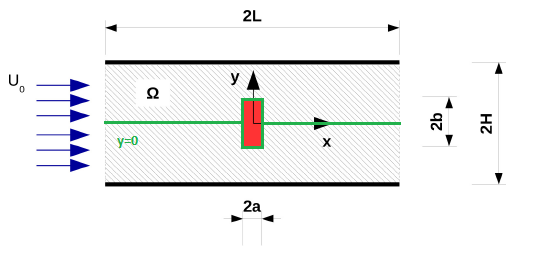
\includegraphics{vitessenulleparoi.png} \end{center}
\vfill\hspace*{0mm}
\caption{Représentation du problème}
\label{Tux}
\end{figure}

\pagebreak

Le problème physique est le suivant :
\begin{itemize} 
   \item Ecoulement incompressible à potentiel dans le canal avec comme dimension $[100\times20]$;
   \item un obstacle au centre du canal [$8\times4$] ;
\end{itemize}

\subsection{Théorie}

L'équation d'équilibre qui régit la fonction de courant $\psi(x,y)$ est l'équation de Laplace en deux dimension.
\begin{center}
$\dfrac{\partial^2\psi}{\partial x^2}+\dfrac{\partial^2\psi}{\partial y^2}=0$
\end{center}

La relation qui relie la vitesse $\overrightarrow{U}$ à la fonction de courant $\psi$ est la suivante:
\begin{center}
$\overrightarrow{U}= \begin{pmatrix}  u \\  v   \end{pmatrix}$ avec $u=\dfrac{\partial \psi}{\partial y}$ et $v=-\dfrac{\partial \psi}{\partial x}$
\end{center}
Les conditions aux limites du problème sont les suivantes:
\begin{itemize} 
   \item Condition à l'entrée du fluide:
	\begin{itemize} 
   	     \item $u(0,y)=U_0$
   	     \item$v(0,y)=0$ 
	\end{itemize}
\end{itemize}
Ces conditions à l'entrée nous permettent de connaitre l'équation de la fonction de courant à l'entrée du canal en intégrant ces deux conditions limites:
\begin{itemize}
	     \item $U_0=\dfrac{\partial \psi}{\partial y}(0,y)$ donc on obtient en intégrant sur y  $\psi(0,y)=U_0y+C(x)$ maintemant il faut déterminer la constante avec la vitesse selon v
	     \item $0=-\dfrac{\partial \psi}{\partial x}$ donc on obtient en intégrant sur x  $C(x)=0$
\end{itemize}

\begin{center}
\fcolorbox{red}{white}{
\begin{minipage}{0.9\textwidth}
Finalement à l'entrée la fonction de Courant vaut $\psi(0,y)=U_0y$
\end{minipage}
}
\end{center}
\begin{itemize}
   \item Condition aux parois du canal :
	\begin{itemize}
	    \item$u(x,0)=0$
	    \item$v(x,0)=0$
	    \item$u(x,20)=0$
	    \item$v(x,20)=0$
	\end{itemize}
Au paroi, la fonction de courant est nulle car y=0, la ligne de courant longe la paroi donc sur la paroi $\psi(x,0)=U_0\times 0$
\pagebreak
\begin{figure}[!h]
\centering
\hspace*{0mm}\vfill
\begin{center} 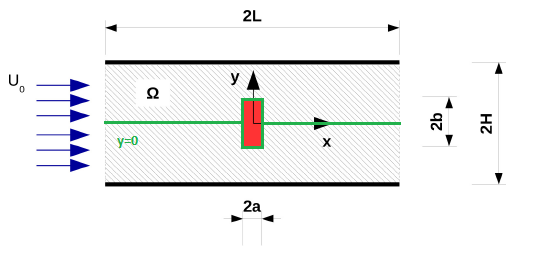
\includegraphics{vitessenulleparoi.png} \end{center}
\vfill\hspace*{0mm}
\caption{Fonction de courant nulle sur l'obstacle}
\label{Tux}
\end{figure}
   \item Condition aux parois de l'obstacle:
	\begin{itemize}
	    \item$\psi(-4,-2)=0$ jusqu'à $\psi(-4,2)=0$
	    \item$\psi(4,-2)=0$ jusqu'à $\psi(4,2)=0$
	    \item$\psi(-4,-2)=0$ jusqu'à $\psi(4,-2)=0$
	    \item$\psi(4,2)=0$ jusqu'à $\psi(4,2)=0$
	\end{itemize}
\end{itemize}
Pour connaitre la pression on utilise l'équation de Bernouilli
\begin{center}
$p+\dfrac{1}{2}\rho U^2+\rho g z=constante$
\end{center}
Dans nos cas, on considère que $z$ varie peu car nous sommes en 2D. Donc l'équation devient:
\begin{center}
$p+\dfrac{1}{2}\rho U^2=constante$
\end{center} 
donc , la différence de la pression est en expression :

\begin{center}
\fcolorbox{red}{white}{
\begin{minipage}{0.8\textwidth}
$$\Delta p=\frac{1}{2}\rho(U^2-U_0^2)=\frac{1}{2}\rho\Big((\frac{\partial\psi}{\partial y})^2+(-\frac{\partial \psi}{\partial x})^2-U_0^2\Big)$$
\end{minipage}
}
\end{center}
\pagebreak
On peut deviner que la vitesse maximum $U_{max}=max(\overrightarrow{U}(x,y))$ quand la vitesse est à la hauteur de l'obstacle.
 En effet, la réduction de l'aire provoque une accélération du flux. C'est d'ailleurs dans cette zone que la pression sera minimum.
\begin{figure}[!h]
\centering
\hspace*{0mm}\vfill
\begin{center} 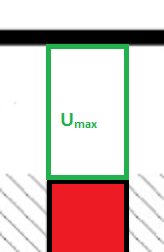
\includegraphics{zonevitessemax.png} \end{center}
\vfill\hspace*{0mm}
\caption{Zone dans laquelle on devrait avoir la vitesse maximun et la pression minimum}
\label{Tux}
\end{figure}

En utilisant l'équation de bernouilli on peut en déduire que la pression est maximale où la vitesse est minimale.

\subsection{Approximation par élément finis}

Pour résoudre le problème, on cherche une solution approchée $\psi_h(x,y)$.
\\
Lors de ce TP, nous allons prendre un maillage triangulaire.
Puis nous allons faire varier le nombre et la positions des degrés de liberté pour les aproximations $P^1, P^2, P^3, P^4, P^5$ sur chaque triangle.
\pagebreak
\begin{figure}[!h]
\centering
\hspace*{0mm}\vfill
\begin{center} 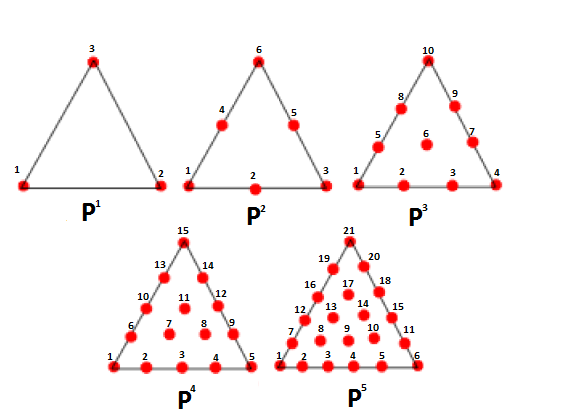
\includegraphics{triangle.png} \end{center}
\vfill\hspace*{0mm}
\caption{Représentation des triangles en fonction du degré d'interpolation}
\label{Tux}
\end{figure}


%%%%%%%%%%%%%%%%%%%%%%%%%%%%%%%%%%%%%%
\section{COMSOL}

\subsection{Etude de écoulement}

Pour créer notre modèle, nous avons d'abord créer un \textbf{assistant de modélisation} "préprogrammé" dans un domaine d'espace \textbf{2D}. Puis nous avons sélectionner un modèle \textbf{mathématiques} car notre écoulement est régi par une \textbf{EDP classique}, en locurrence ici \textbf{l'équation de Laplace}.\\

La variable dépendante est \textbf{$\psi$} qui est un \textbf{potentiel de vitesse ($m^2/s$)} sans terme source. L'étude est \textbf{stationnaire}

\subsection{Création du domaine d'écoulement}

\begin{itemize}
    \item[$\bullet$]On crée les parois extérieur , clic droit en \textbf{Géométrie} , ensuite clic gauche en \textbf{rectangle} , et on crée une domaine rectanglulaire avec l'origine au centre du rectangle,de largeur $2L=100$ et hauteur $2H=20$ et on construit la sélection .
    \item[$\bullet$]On crée l'obstacle , clic droit en \textbf{Géométrie} , ensuite clic gauche en \textbf{rectangle} , et on crée une domaine rectanglulaire avec l'origine au centre du rectangle,de largeur $2a=8$ et hauter $2b=4$ .
    \item[$\bullet$]On fait la différence entre les deux rectangles , clic droit en \textbf{Géométrie} , ensutie clic gauche en \textbf{Booléens et partitions},puis on fait la \textbf{différence}. Puis on soustrait le rectangle obstacle au rectangle du domaine.
\end{itemize}

\subsection{Prise en compte des conditions limites}

\begin{itemize}
    \item[$\bullet$] On ajoute les Conditions limites sur les parois . On clique  droite sur \textbf{Equation de Laplace} , ensuite clic gauche en \textbf{Conditions Dirichlet} , puis on choisi les frontières des parois extérieurs du domaine et on impose que $\psi=U_0y$.
    \item[$\bullet$] Pour les conditions limites sur l'obstacle , on choisi les bords d'obstacle en fonction : $\psi=0$.
    \item[$\bullet$]Clic gauche en \textbf{Construireselctions} .
\end{itemize}

\subsection{Changement de maillage}

\begin{itemize}
    \item[$\bullet$]on peut créer un \textbf{maillage} controlé par la physique et après on choisi la \textbf{taille de l'élément}
    \item[$\bullet$] on peut aussi créer un \textbf{maillage controlé par l'utilisateur}, à ce moment là, on peut modifié la \textbf{taille} en changeant la taille d'élément maximale
\end{itemize}

Ensuite, on réalise l'\textbf{étude} avec le bouton calculer, il est nécessaire de recalculer à chaque fois que l'on modifie le maillage.

\subsection{Création d'un graphique iso-contours}

\begin{itemize}
    \item[$\bullet$]pour crée un graphique iso contours, on clique droit sur\textbf{Résultats} puis sur \textbf{groupe de graphique 2D}. On clique droit sur le groupe de graphique 2D qu'on a crée et on clic sur \textbf{isovaleur}, on choisi dans expression ce qu'on veut visualiser avec les isovaleur
    \item[$\bullet$] il est possible de modifié les lignes de niveaux dans \textbf{niveaux}
    \item[$\bullet$]on peut aussi afficher les \textbf{valeurs} pour chaque ligne d'isovaleur
\end{itemize}

\subsection{Création d'un profil de vitesse}

\begin{itemize}
    \item[$\bullet$]Pour créer un profil de vitesse, on crée un autre \textbf{groupe de graphique 2D} puis on clic droit sur ce groupe de graphique 2D et on choisit \textbf{surface}
    \item[$\bullet$] on choisit dans l'expression de $u$ avec $u=\dfrac{\partial psi}{\partial y}$
\end{itemize}

\subsection{Calcul d'une grandeur physique en un point}

\begin{itemize}
    \item[$\bullet$] d'abord, on crée un point avec \textbf{géométrie}, on choisit \textbf{point} et on le place où on a besoin de connaitre la grandeur physique, on entre l'abscisse et l'ordonnée.
    \item[$\bullet$]on clique droit \textbf{Résultat}, on choisit \textbf{groupe de graphique 1D}, on donne l'expression de la grandeur qu'on veut mesurer
    \item[$\bullet$]on clique droit sur le \textbf{groupe de graphique 1D} qu'on vient de créer on sélectionne \textbf{graphique ponctuel} puis on choisit le point qu'on a crée précédemment pour mesurer la grandeur physique à cette endroit.
\end{itemize}

\subsection{Changement du type d'approximation}

\begin{itemize}
    \item[$\bullet$]pour changer le type d'interpolation on clic droit sur \textbf{Equation de Laplace}, on choisit \textbf{global} puis on clique sur \textbf{discrétisation}. Enfin on choisit sur ordre d'élement si on veut P1 on prend linéaire, si on veut P2 on prend quadratique, si on veut P3 on prend Cubique, si on veut P4 on choisit quartique et si on veut P5 on choisit Quintique.

\end{itemize}


%%%%%%%%%%%%%%%%%%%%%%%%%%%%%%%%%%%%%%%%%%
\section{Résultats}


%%%%%%%%%%%%%%%%%%%%%%%%%%%%
\subsection{Maillage}
\subsubsection{Maillage physique fin}
\begin{figure}[!h]
\centering
\hspace*{0mm}\vfill
\begin{center} 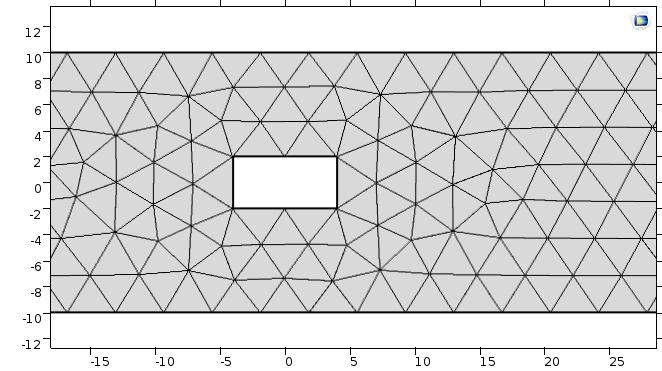
\includegraphics[width=1.\textwidth]{maillagefin.jpg} \end{center}
\vfill\hspace*{0mm}
\caption{Maillage physique plus extra fin sans segements }
\label{maillage_physique}
\end{figure}
Dans le figure \ref{maillage_physique} , on présent les maillages avec triangles . Ce que on utilise en élément finis .
\pagebreak
\subsubsection{Maillage physique extra fin}
\begin{figure}[!h]
\centering
\hspace*{0mm}\vfill
\begin{center} 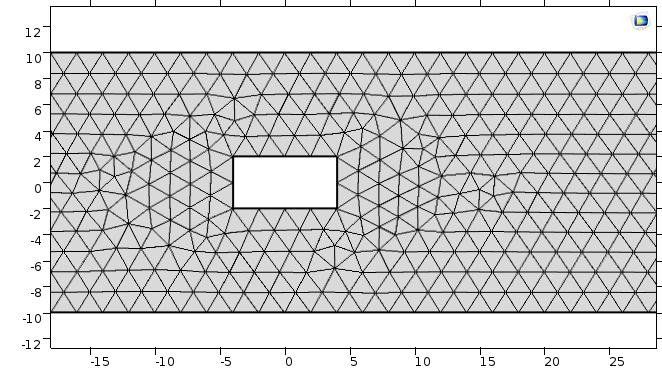
\includegraphics[width=1.\textwidth]{maillagextrafin.jpg} \end{center}
\vfill\hspace*{0mm}
\caption{Maillage physique plus extra fin sans segements }
\label{maillage_physique}
\end{figure}\pagebreak
Dans le figure \ref{maillage_physique} , on présent les maillages avec triangles . Ce que on utilise en élément finis .

\subsubsection{Maillage défini par taille d'élé maxi hh avec segments}
\begin{figure}[!h]
\centering
\hspace*{0mm}\vfill
\begin{center} 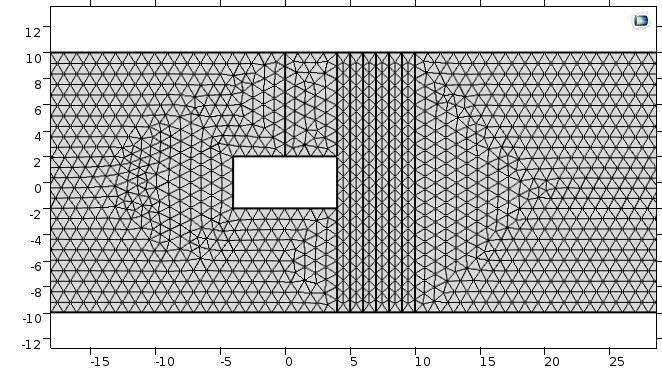
\includegraphics[width=1.\textwidth]{maillagehh1.jpg} \end{center}
\vfill\hspace*{0mm}
\caption{Maillage distance maxi hh  }
\label{maillage_hh}
\end{figure}
Dans le figure \ref{maillage_hh} , on défini les maillages par utilisateur , on fait la distance maximale .....est hh , et on consduis le sélection .
 
 
\subsubsection{Maillage défini par distance maxi 5*hh}
\begin{figure}[!h]
\centering
\hspace*{0mm}\vfill
\begin{center} 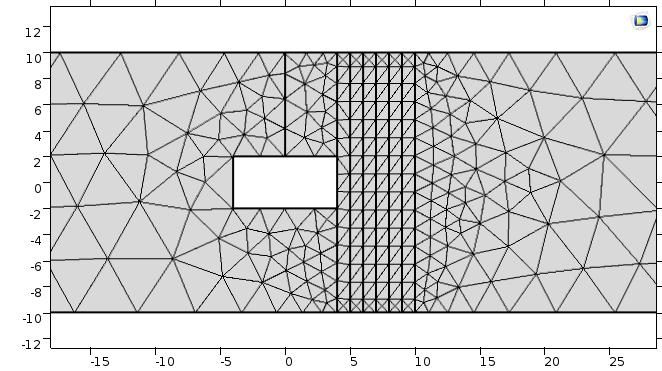
\includegraphics[width=1.0\textwidth]{maillage5hh1.jpg} \end{center}
\vfill\hspace*{0mm}
\caption{Maillage distance maxi 5*hh  }
\label{maillage_5hh}
\end{figure}\pagebreak
Dans le figure \ref{maillage_5hh} , on défini les maillages par utilisateur , on change la distance maximale .....est 5*hh , et on consduis le sélection . On trouve que quand on augemente la distance , nombre des triangles diminue . 


%%%%%%%%%%%%%%%%%%%%%%%%%%
\subsection{Fonction de courant}
\subsubsection{Profie de fonction de courant}
\begin{figure}[!h]
\centering
\hspace*{0mm}\vfill
\begin{center} 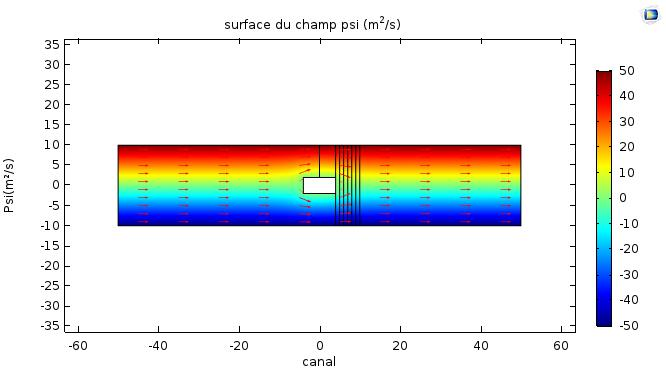
\includegraphics[width=1.\textwidth]{psi_surface.jpg} \end{center}
\vfill\hspace*{0mm}
\caption{Fonction de courant tous les points surface }
\label{phi_surface}
\end{figure}\pagebreak
Dans le figure \ref{phi_surface} , on présent les fonctions de courants pour tous les points dans la région et on fait flèches sur surface . On peut trouver que suivant le direction $\overrightarrow{x}$ la fonction de courant est uniforme ; suivant le direction $\overrightarrow{y}$ la fonction de courant augmente linéaire ; autour l'obstacle ,  la fonction de courant est nulle . Ces résultats est bien verifié les conditions limites . 


\subsubsection{isole profie de fonction de courant}
\begin{figure}[!h]
\centering
\hspace*{0mm}\vfill
\begin{center} 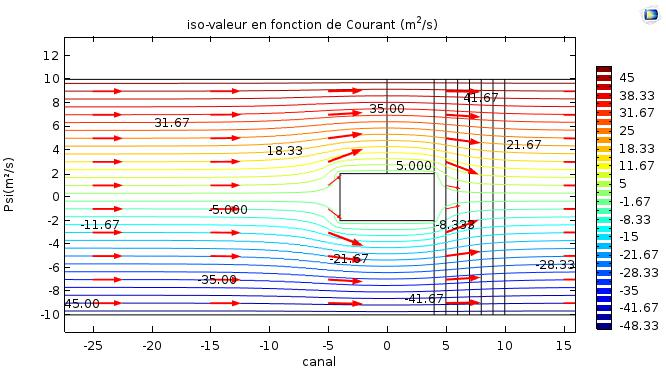
\includegraphics[width=1.\textwidth]{iso_psi_surface.jpg} \end{center}
\vfill\hspace*{0mm}
\caption{isovaleur de fonction de courant tous les points surface }
\label{phi_surface_iso}
\end{figure}\pagebreak
Dans le figure \ref{phi_surface_iso} , on isoles les fonctions de courants pour tous les points dans la région et on fait flèches sur surface . On a minimisation de fonction de courant sur les deux parois .  Autour l'obstacle ,  la fonction de courant est zero  . 




%%%%%%%%%%%%%%%%%%%%%%%%%%
\subsection{Différence de pression}
\subsubsection{Profie de différence de pression}
\begin{figure}[!h]
\centering
\hspace*{0mm}\vfill
\begin{center} 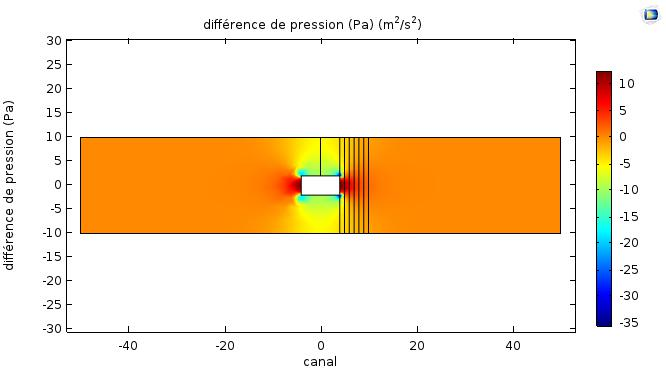
\includegraphics[width=1.\textwidth]{pression_surface.jpg} \end{center}
\vfill\hspace*{0mm}
\caption{Champ de différence de pression  }
\label{pression_surface}
\end{figure}\pagebreak
Dans le figure \ref{pression_surface} , on présent la différence de pression entre le ponit on etude et le point d'entré  . On a pression uniforme dans les région loin d'obstacle . On peut trouver que dans les deux cotés d'obstacle $(a,\pm b)$, la différence de la presssion est minimale . Dans le mid de la frontière dernière $(a,0)$on trouve la différence de la pression est maximale . 


\subsubsection{isole profie de différence de pression}
\begin{figure}[!h]
\centering
\hspace*{0mm}\vfill
\begin{center} 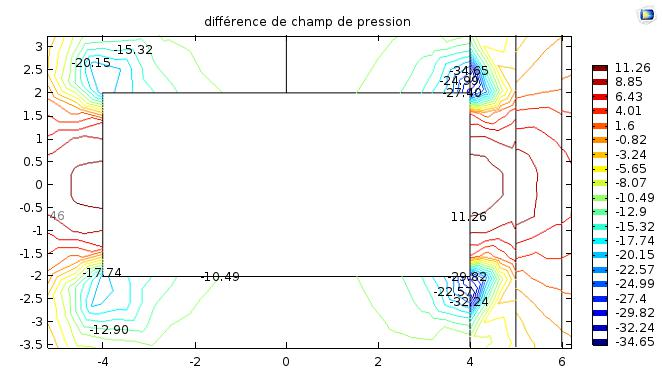
\includegraphics[width=1.\textwidth]{iso_pression_surface.jpg} \end{center}
\vfill\hspace*{0mm}
\caption{isovaleur de champ de différence de pression }
\label{pression_surface_iso}
\end{figure}\pagebreak
Dans le figure \ref{pression_surface_iso} , on isoles les fonctions de courants pour tous les points dans la région et on fait agrandir la région autour d'obstacle  . 

\subsubsection{Différence de pression dans le segements}
\begin{figure}[!h]
\centering
\hspace*{0mm}\vfill
\begin{center} 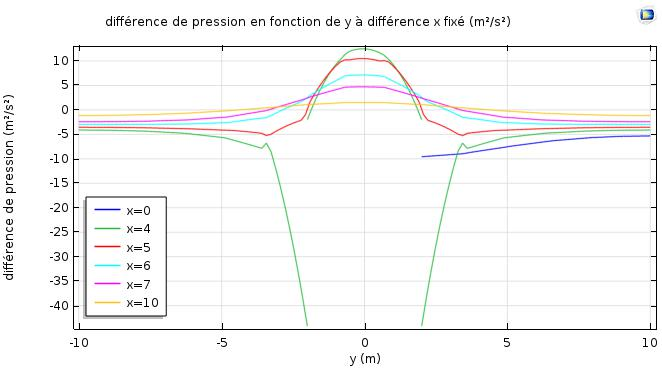
\includegraphics[width=1.\textwidth]{pression_segment.jpg} \end{center}
\vfill\hspace*{0mm}
\caption{pression dans le point 1 }
\label{pression_ponctuel1}
\end{figure}\pagebreak
Dans le figure \ref{pression_ponctuel1} , on i...........................................................................

\subsubsection{Precisions différence de pression dans le segements}
\begin{figure}[!h]
\centering
\hspace*{0mm}\vfill
\begin{center} 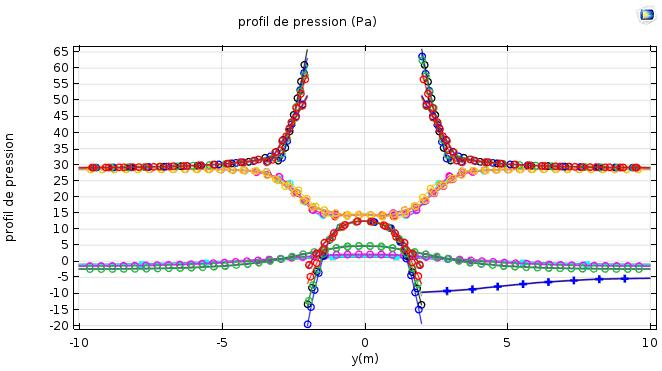
\includegraphics[width=1.\textwidth]{pre_pression_segment.jpg} \end{center}
\vfill\hspace*{0mm}
\caption{pression dans le point 1 }
\label{pression_ponctuel1}
\end{figure}\pagebreak
Dans le figure \ref{pression_ponctuel1} , on i..........................................................................



\subsubsection{Detail pression dans le segments}
\begin{figure}[!h]
\centering
\hspace*{0mm}\vfill
\begin{center} 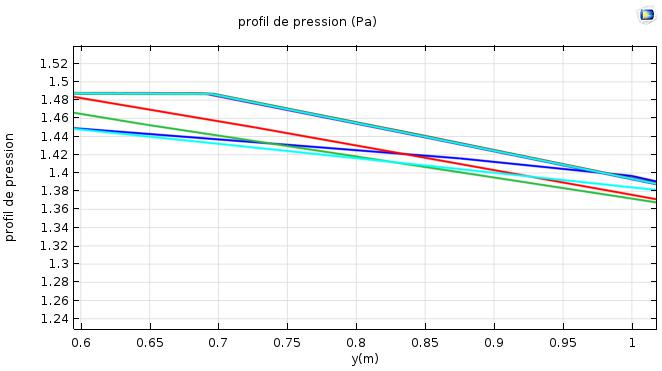
\includegraphics[width=1.\textwidth]{pression_seg_detail.jpg} \end{center}
\vfill\hspace*{0mm}
\caption{pression dans le point 1 }
\label{detail_pression}
\end{figure}\pagebreak
Dans le figure \ref{detail_pression} , on

\subsubsection{Différence de pression ponctuel}
\begin{figure}[!h]
\centering
\hspace*{0mm}\vfill
\begin{center} 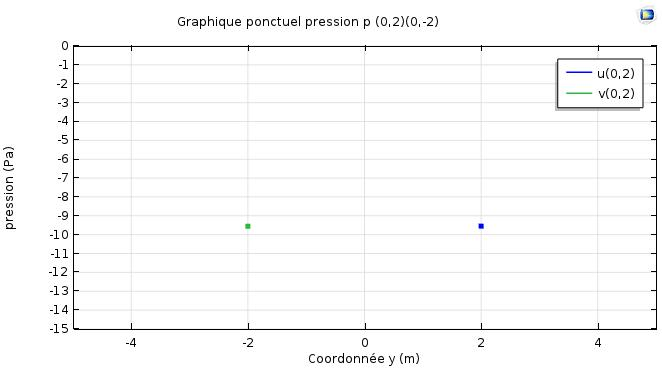
\includegraphics[width=1.\textwidth]{pression_ponctuel.jpg} \end{center}
\vfill\hspace*{0mm}
\caption{pression dans le point 1 }
\label{pression_ponctuel1}
\end{figure}\pagebreak
Dans le figure \ref{pression_ponctuel1} , on i..........................................................................






%%%%%%%%%%%%%%%%%%%%%%%%%%
\subsection{Profie de vitesse u}
\subsubsection{Profie de vitesse surface}
\begin{figure}[!h]
\centering
\hspace*{0mm}\vfill
\begin{center} 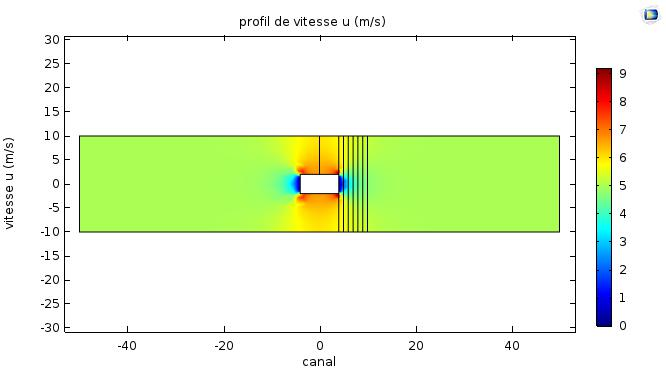
\includegraphics[width=1.\textwidth]{u_surface.jpg} \end{center}
\vfill\hspace*{0mm}
\caption{Vitesse horizontale surface}
\label{vitesse_u}
\end{figure}\pagebreak
Dans le figure \ref{vitesse_u} , on présent la profie de vitesse horizontale $u$ . On a vitesse uniforme $u_0$ dans les région loin d'obstacle . On peut trouver que dans les quatres cotés d'obstacle $(\pm a,\pm b)$, la vitesse horizontale est maximale et symétrique.  


\subsubsection{isole profie de vitesse horizontale surface}
\begin{figure}[!h]
\centering
\hspace*{0mm}\vfill
\begin{center} 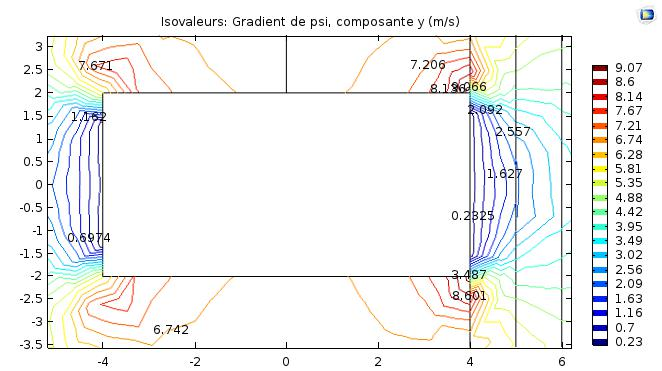
\includegraphics[width=1.\textwidth]{iso_u_surface.jpg} \end{center}
\vfill\hspace*{0mm}
\caption{isovaleur de champ de profie de vitess u}
\label{vitesse_u_iso}
\end{figure}\pagebreak
Dans le figure \ref{vitesse_u_iso} , on isoles la profie de vitesse $u$ pour tous les points dans la région et on fait agrandir la région autour d'obstacle pour bien affiché . 


\subsubsection{Profie de vitesse horizontale sur les segements }
\begin{figure}[!h]
\centering
\hspace*{0mm}\vfill
\begin{center} 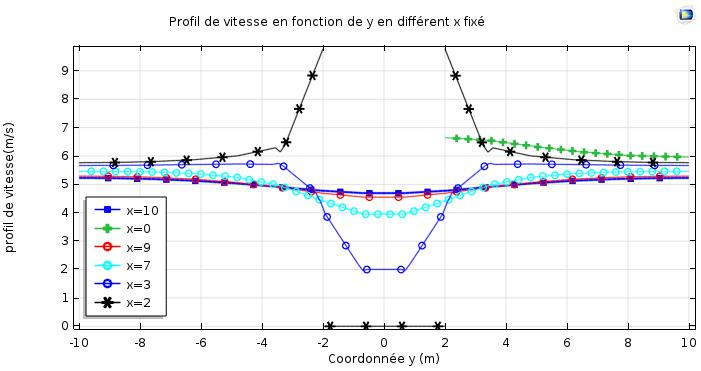
\includegraphics[width=1.\textwidth]{u_segment.jpg} \end{center}
\vfill\hspace*{0mm}
\caption{Vitesses horizontales sur les segements}
\label{vitesse_u_sege}
\end{figure}\pagebreak
Dans le figure \ref{vitesse_u_sege} , on présent la fonction de vitesse $u$ dans les segements . 


\subsubsection{Précisions profie de vitesse horizontale sur les segements }
\begin{figure}[!h]
\centering
\hspace*{0mm}\vfill
\begin{center} 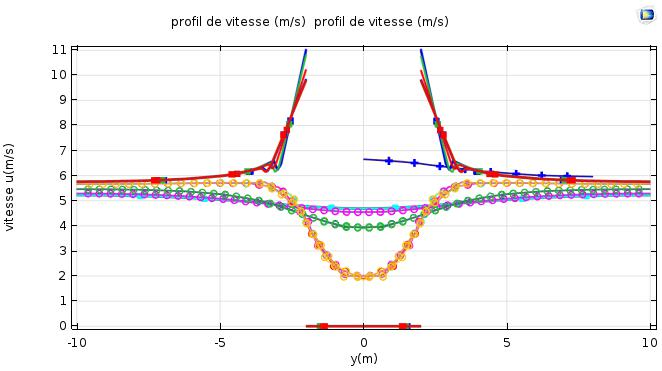
\includegraphics[width=1.\textwidth]{pre_u_segment.jpg} \end{center}
\vfill\hspace*{0mm}
\caption{Vitesses horizontales sur les segements  avec precisions}
\label{vitesse_u_sege_hh}
\end{figure}\pagebreak
Dans le figure \ref{vitesse_u_sege_hh} , on présent la fonction de vitesse $u$ dans les segements . 

\subsubsection{Detail de vitesse horizontale sur les segments }
\begin{figure}[!h]
\centering
\hspace*{0mm}\vfill
\begin{center} 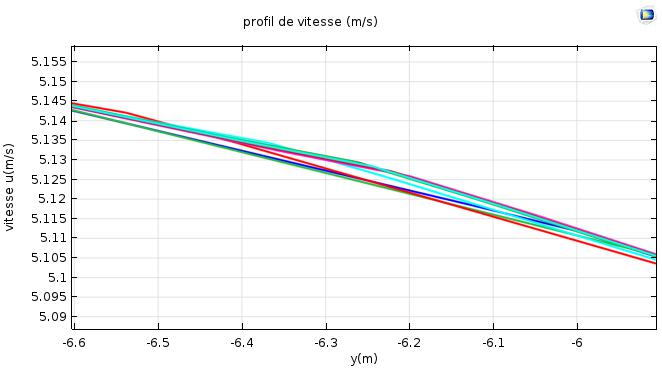
\includegraphics[width=1.\textwidth]{u_seg_detail.jpg} \end{center}
\vfill\hspace*{0mm}
\caption{Detail de vitesse horizontale sur la segment x=10}
\label{detail_vitesse_u_seg}
\end{figure}\pagebreak
Dans le figure \ref{detail_vitesse_u_seg} , on présent la fonction de vitesse $u$ dans les segements . 

\subsubsection{Vitesse horizontale ponctuel }
\begin{figure}[!h]
\centering
\hspace*{0mm}\vfill
\begin{center} 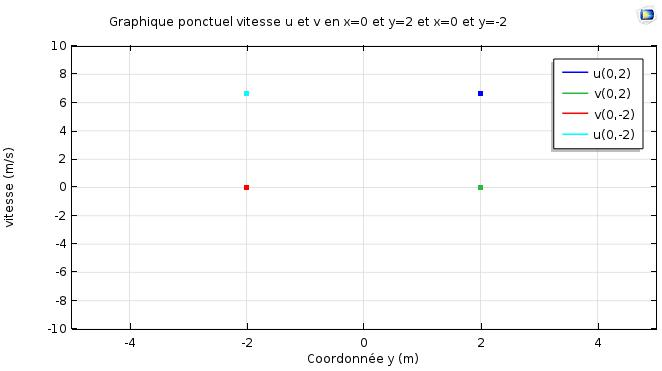
\includegraphics[width=1.\textwidth]{u_v_ponctuel.jpg} \end{center}
\vfill\hspace*{0mm}
\caption{vitesse horizontale ponctuel}
\label{u_ponctuel}
\end{figure}\pagebreak
Dans le figure \ref{u_ponctuel} , on i---------------------------------------------------------------------------

%%%%%%%%%%%%%%%%%%%%%%%%%%
\subsection{Profie de vitesse v}
\begin{figure}[!h]
\centering
\hspace*{0mm}\vfill
\begin{center} 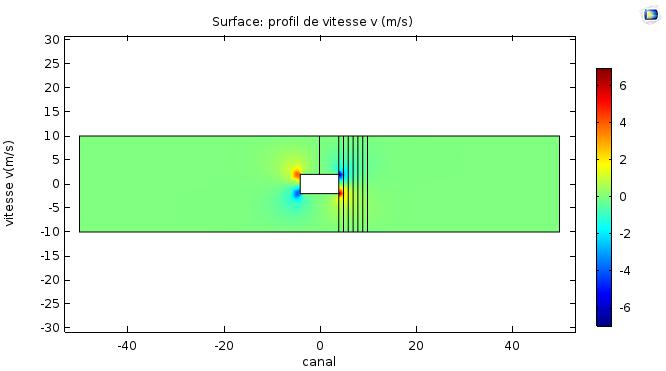
\includegraphics[width=1.\textwidth]{v_surface.jpg} \end{center}
\vfill\hspace*{0mm}
\caption{Vitesse verticale surface }
\label{vitesse_v}
\end{figure}\pagebreak
Dans le figure \ref{vitesse_v} , on présent la profie de vitesse horizontale $v$ . On a vitesse uniforme $0$ dans les région loin d'obstacle . On peut trouver que dans les quatres cotés d'obstacle $(\pm a,\pm b)$, la vitesse horizontale est maximale et antisymétrique .  

\subsubsection{Profie de vitesse verticale surface}
\begin{figure}[!h]
\centering
\hspace*{0mm}\vfill
\begin{center} 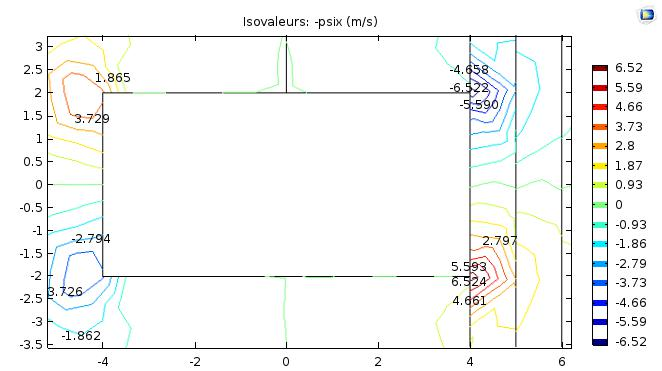
\includegraphics[width=1.\textwidth]{iso_v_surface.jpg} \end{center}
\vfill\hspace*{0mm}
\caption{isovaleur de champ de vitesse verticale v}
\label{vitesse_v_iso}
\end{figure}\pagebreak
Dans le figure \ref{vitesse_v_iso} , on isoles la profie de vitesse $v$ pour tous les points dans la région et on fait agrandir la région autour d'obstacle pour bien affiché . 

\subsubsection{Profie de vitesse verticale sur les segements }
\begin{figure}[!h]
\centering
\hspace*{0mm}\vfill
\begin{center} 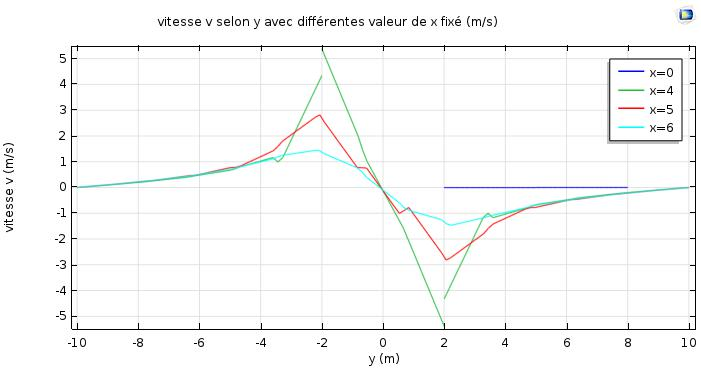
\includegraphics[width=1.\textwidth]{v_segment.jpg} \end{center}
\vfill\hspace*{0mm}
\caption{Vitesses verticales sur les segements}
\label{vitesse_v_sege}
\end{figure}\pagebreak
Dans le figure \ref{vitesse_v_sege} , on présent la fonction de vitesse $u$ dans les segements . 



\subsubsection{Précisions profie de vitesse verticale sur les segements }
\begin{figure}[!h]
\centering
\hspace*{0mm}\vfill
\begin{center} 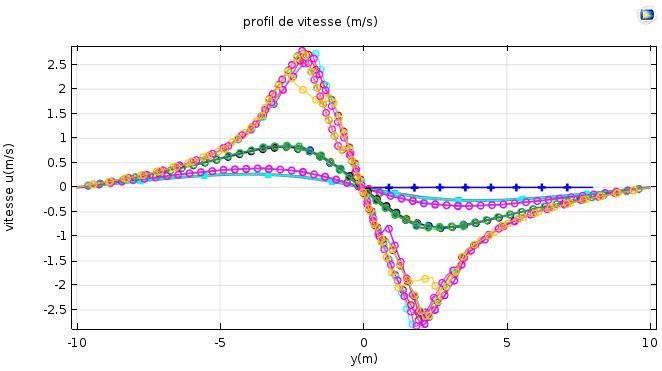
\includegraphics[width=1.\textwidth]{pre_v_segment.jpg} \end{center}
\vfill\hspace*{0mm}
\caption{Vitesses verticales sur les segements avec precisions}
\label{vitesse_v_sege_hh}
\end{figure}\pagebreak
Dans le figure \ref{vitesse_v_sege_hh} , on présent la fonction de vitesse $v$ dans les segements . 


\subsubsection{Detail de vitesse verticale sur les segments }
\begin{figure}[!h]
\centering
\hspace*{0mm}\vfill
\begin{center} 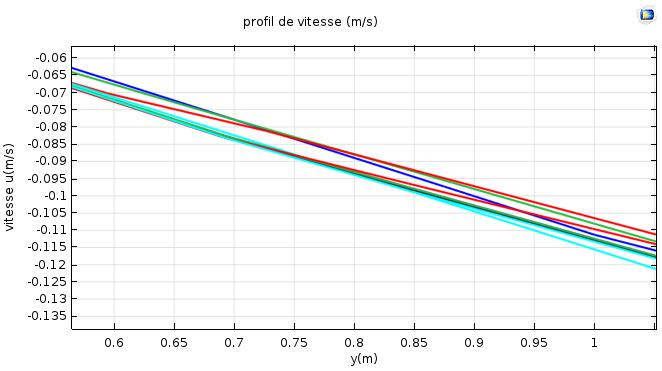
\includegraphics[width=1.\textwidth]{v_seg_detail.jpg} \end{center}
\vfill\hspace*{0mm}
\caption{Detail de vitesse verticale sur les segments}
\label{detail_vitesse_v_seg}
\end{figure}\pagebreak
Dans le figure \ref{detail_vitesse_v_seg} , on présent la fonction de vitesse $v$ dans les segements . 


\subsubsection{Vitesse verticale ponctuel }
\begin{figure}[!h]
\centering
\hspace*{0mm}\vfill
\begin{center} 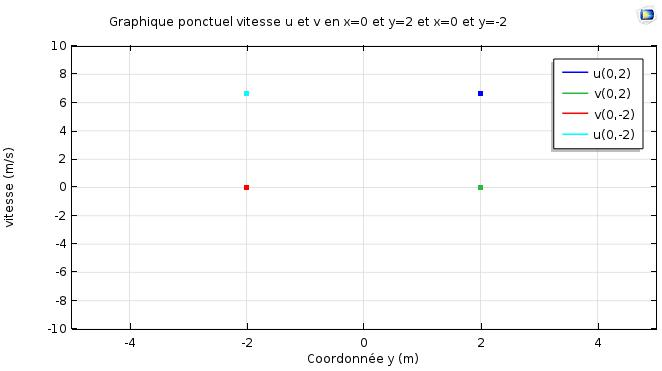
\includegraphics[width=1.\textwidth]{u_v_ponctuel.jpg} \end{center}
\vfill\hspace*{0mm}
\caption{vitesse verticale ponctuel }
\label{v_ponctuel}
\end{figure}\pagebreak
Dans le figure \ref{v_ponctuel} , on ----------------------------------



%%%%%%%%%%%%%%%%%%%%%%%%%%%%%
\subsection{Changement l'ordre d'élément}

\subsubsection{P1}.........................
\begin{figure}[!h]
\centering
\hspace*{0mm}\vfill
\begin{center} 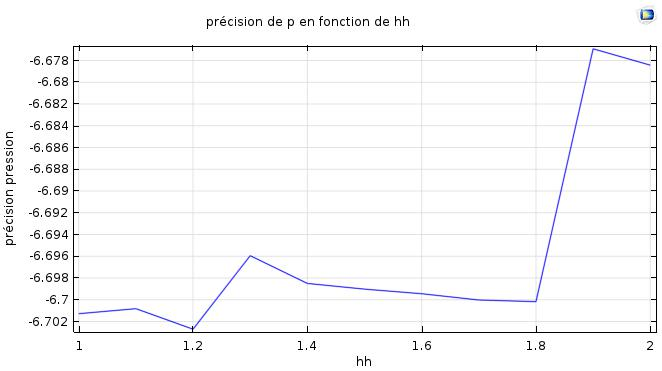
\includegraphics[width=1.\textwidth]{pression_P1.jpg} \end{center}
\vfill\hspace*{0mm}
\caption{pression-P1 }
\label{v_ponctuel}
\end{figure}\pagebreak

\begin{figure}[!h]
\centering
\hspace*{0mm}\vfill
\begin{center} 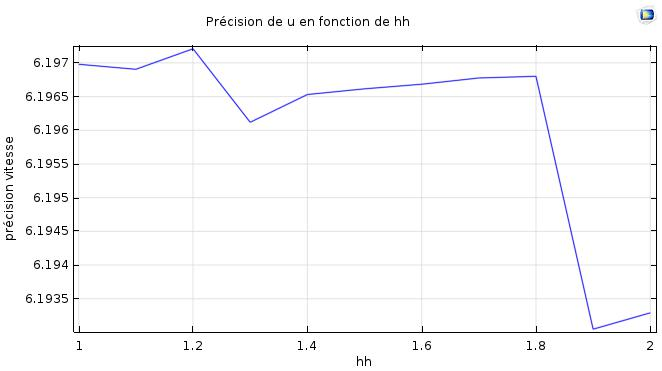
\includegraphics[width=1.\textwidth]{vitesse_u_P1.jpg} \end{center}
\vfill\hspace*{0mm}
\caption{vitesse-P1 }
\label{v_ponctuel}
\end{figure}\pagebreak

\subsubsection{P2}.....................

\begin{figure}[!h]
\centering
\hspace*{0mm}\vfill
\begin{center} 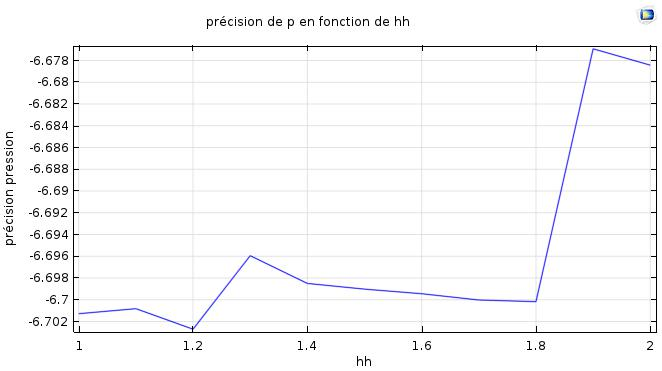
\includegraphics[width=1.\textwidth]{pression_P2.jpg} \end{center}
\vfill\hspace*{0mm}
\caption{pression-P2 }
\label{v_ponctuel}
\end{figure}\pagebreak

\begin{figure}[!h]
\centering
\hspace*{0mm}\vfill
\begin{center} 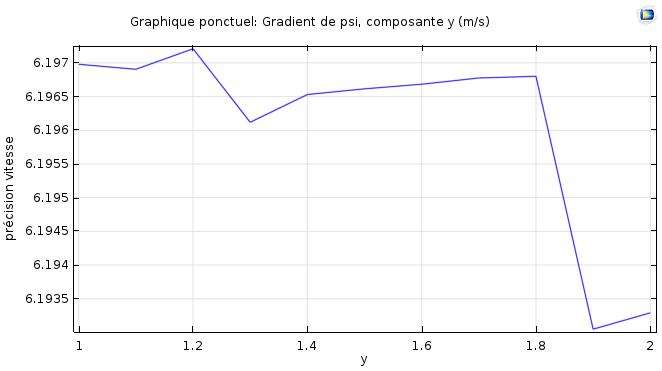
\includegraphics[width=1.\textwidth]{vitesse_u_P2.jpg} \end{center}
\vfill\hspace*{0mm}
\caption{vitesse-P2 }
\label{v_ponctuel}
\end{figure}\pagebreak
\subsubsection{P3}.........................

\begin{figure}[!h]
\centering
\hspace*{0mm}\vfill
\begin{center} 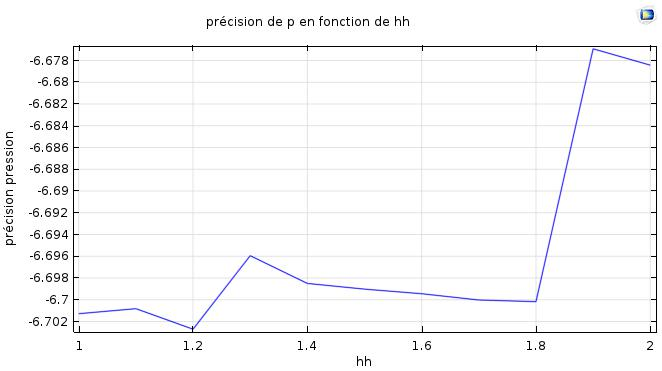
\includegraphics[width=1.\textwidth]{pression_P3.jpg} \end{center}
\vfill\hspace*{0mm}
\caption{pression-P3 }
\label{v_ponctuel}
\end{figure}\pagebreak
\begin{figure}[!h]
\centering
\hspace*{0mm}\vfill
\begin{center} 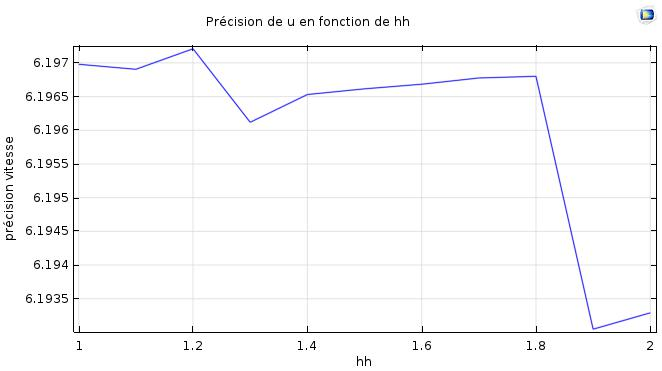
\includegraphics[width=1.\textwidth]{vitesse_u_P3.jpg} \end{center}
\vfill\hspace*{0mm}
\caption{vitesse-P3 }
\label{v_ponctuel}
\end{figure}
Nous trouvons que la vitesse et la pression suivant $P^1$,$P^2$,$P^3$ est la même. Cela veut dire que notre précision est déjà trop grande pour voir une différence suivant le polynôme d'interpolation.













\pagebreak
%%%%%%%%%%%%%%%%%%%%%%%%%%%%%%%%%%%%%%%%%
\section{Conclusions}

Lors de ce TP, nous avons appris à utiliser le logiciel \textbf{COMSOL}, notamment en créant un domaine d'écoulement qui dépend d'une équation ( l'équation de Laplace) et non du type d'écoulement ( ce que nous avons pu voir dans un précédent TP avec M.SPELT où l'étude était basé sur un écoulement à régime laminaire).\\

Le principal objectif de ce TP était de calculer la vitesse dans l'écoulement ainsi que la pression et de la comparer avec les résultats obtenu en théorie pour savoir si nos hypothéses était correcte. Ensuite nous avons étudiés les conséquence du changement de maillage, pour un maillage assez gros nous avons pu remarqué que les différences entre les courbes était importantes. Puis, en affinant un peu plus nous avions des courbes proches les une des autres assez rapidement.\\

Ensuite, nous avons changer le type d'interpolation avec un maillage grossier et fin et nous avons remarquer que si nous prenions un degré d'interpolation assez important il n'était pas nécessaire de prendre un maillage très fin car la précision de notre modèle ne variait pas énormément. De même si on prend un maillage extra fin, il n'est pas nécessaire de prendre un degré d'interpolation très élevé ($P^1$ étant suffisant dans ce cas).\\

Enfin, suite à notre TP, il serait possible d'étudié la fonction de courant suivant différents type d'obstacle pour savoir si la forme ou l'allure de l'obstacle influe sur la vitesse et la pression et si oui de quelle manière. Nous pourrions aussi changer la viscosité pour savoir si la variation de vitesse et de pression serait toujours aussi grande aux points critique.



%\bibliography{MonBiblio.bib}
%\bibliographystyle{unsrtnat}	
\end{document}
